% !TeX encoding=utf8
% !TeX program = pdflatex
% !BIB = biber

\listfiles % listet alle geladenen Pakete im .log file
% sollte ihr .tech-file nicht kompilieren, so vergleichen Sie bitte Ihre Liste
% mit PaketListe.txt

\documentclass[paper=a5,
      fontsize=10pt,
      parskip=half-, %
      ngerman   % Neue Rechtschreibung, d.\,h. (Silbentrennung)
]{scrartcl}

\usepackage{packages} % Präambel laden
% NOTE selbstgemacht...
\newcommand\name[1]{\texttt{#1}}
\usepackage{float}
\usepackage{subcaption}
% NOTE selbstgemacht ende

% Laden der .bib Datei
\addbibresource{document.bib}

% TITEL des Beitrags % \LARGE zur Erzeugung korrekter Überschriftengröße
\title{\LARGE{Automatische Klassifizierung handgezeichneter Mechanismen durch maschinelles Lernen
}}

% AUTOREN (Vorname, Nachname)
\author{Stefan Gössner*, Kai Lawrence**}

% DATUM ausblenden
\date{}

% dieses Feld wird benutzt um die Kontaktadresse darzustellen
% bitte nutzen sie ein hochgestellten Stern (*) um bei mehreren Instituten zu
%unterscheiden
\publishers{* FH Dortmund, Professur für Dynamik, Mechnanismentechnik und Webtechnologien\\
	stefan.gössner@fh-dortmund.de
\\ \vspace{\baselineskip}
% Bei mehreren Instituten nutzen Sie bitte mehrere hochgestellte Sterne, um die
%Autoren zuzuordnen
** FH Dortmund, Maschinenbaustudent\\
	kaihenning.lawrence002@stud.fh-dortmund.de}


\begin{document}

% Wahl der Sprache des Dokuments (ngerman oder englisch)
\selectlanguage{ngerman}

\maketitle % erzeuge Titel

\section*{Kurzfassung}
Für eine schnelle, digitale Skizze zweidimensionaler Mechanismen erlauben neue Technologien im Vergleich zu aktuellen Methoden komfortablere Formen der Benutzerinteraktion.
Es gibt zwar bereits Anwendungen zur schnellen und intuitiven Erstellung von Mechanismen, aber für kurze Betrachtungen ist der Einsatz solcher Editoren in vielen Fällen nicht der Mühe wert.

Um auch ad-hoc eine Möglichkeit zu haben, Mechanismen interaktiv oder animierbar zu betrachten, wird nun ein Programm entwickelt, welches es ermöglichen soll, Handzeichnungen zu scannen und den respektiven Mechanismus digital zu ermitteln.

\section*{Abstract}
For fast, digital sketching of two-dimensional mechanisms, new technologies allow more comfortable forms of user interaction compared to current methods.
Although there are already applications for the fast and intuitive creation of mechanisms, for brief observations the use of such editors is in many cases not worth the effort.

In order to be able to view mechanisms interactively or animatedly on an ad-hoc basis, a program is now being developed which will allow hand drawings to be scanned and the respective mechanism to be determined digitally.


\section{Introduction}

This project builds upon work previously done to learn the fundamentals of machine learning, which can be found at \url{aka.klawr.de/srp}.
The target was to introduce machine learning in to the field of kinematics mainly undertaken in web environment by creating a statistical model to classify handwritten mechanical symbols.

In this project this idea is taken further to detect whole mechanisms by determining the position of the symbols in unspecialized pictures\footnote{The data used to train the symbol classifier assumes symbols which are centered and fill the whole picture}.

After localization is done, the next problem is to detect the connections between nodes.
For this the images between nodes have to be cropped and processed to be able to get a reasonable prediction.
A new inference model is trained to classify these processed images to their respective constraint counterpart.

The resulting coordinates and labels are converted into \name{mec2} nodes and constraints as JSON-string.
This conversion makes it possible to convert the gathered information and make them processable for physic engines like \name{mec2}.
The creation of these JSON-strings is then tested in various environments.

A \name{Progressive Web App}(PWA) is created to nest this new functionality into an application.
For this the inference models are transformed to work in JavaScript to be able to make predictions from within other environments.

The \name{mec2} HTML element is embedded into this app to be able to apply detected nodes and constraints to a mechanical linkage.
This PWA is able to edit the mechanical linkage itself and implements the \name{mec2} API to offer all features the \name{mec2} HTML element does.

The PWA is then used as frontend for different implementations using WPF and WinUI.
These applications explore the possibility of linking the model to other programming languages, like C++, to improve performance.
Other ideas like communication between the PWA and a webserver to get better performance are also explored.


\section{Was erkannt werden soll}
\name{mec-2} modelliert Mechanismen durch
sogenannte \name{Nodes} und \name{Constraints}.
Die Gelenke sind entsprechend als Nodes und Glieder als Constraints zu betrachten.
Beispielhaft für ein Viergelenk sähe das generierte JSON gemä{\ss} Abbildung \ref{fig:4bar} aus.

\begin{figure}
  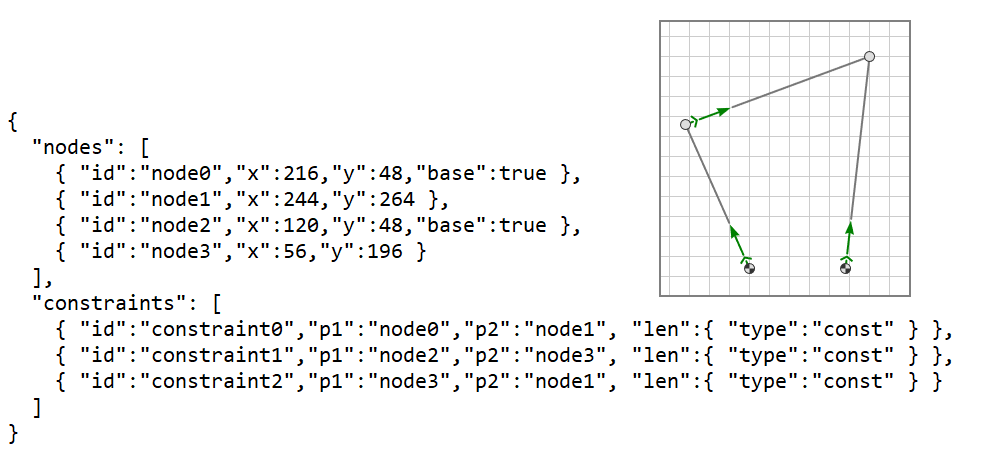
\includegraphics[width=\textwidth]{images/4bar_json}
  \caption{Die JSON-Darstellung eines durch mec-2 erstellten Viergelenks mit dem entsprechend generierten Mechanismus.}
  \label{fig:4bar}
\end{figure}

Um diesen Mechanismus durch eine Handzeichnung zu erstellen, ist es erforderlich, einen Algorithmus zu trainieren, der in der Lage ist, mit einer entsprechenden Skizze als Input solchen JSON-Code als Output zu produzieren.

Hierfür mussten zunächst Trainingsdaten geschaffen werden, anhand derer ein solcher Algorithmus Merkmale erlernen kann, die eine Zuordnung der Eingangsbilder zu den entsprechenden Lösungen bilden kann.
Es wurden etwa 1200 Nodes, 1200 Base-Nodes und 1200 nicht zutreffende Bilder erstellt, welche vor dem Training durch Rotation und Spiegelung augmentiert wurden, um die Varianz der Trainingsdaten zu erhöhen.

Des Weiteren wurden von \name{mec-2} genutzte Symbole dem Trainingsset hinzugefügt, sodass der Algorithmus diese nicht als Nodes erkennt, damit Mechanismen erweitert werden können, ohne die bereits erkannten Elemente nochmal zu erkennen.

\begin{figure}
  \centering
    \begin{subfigure}[b]{0.4\textwidth}
        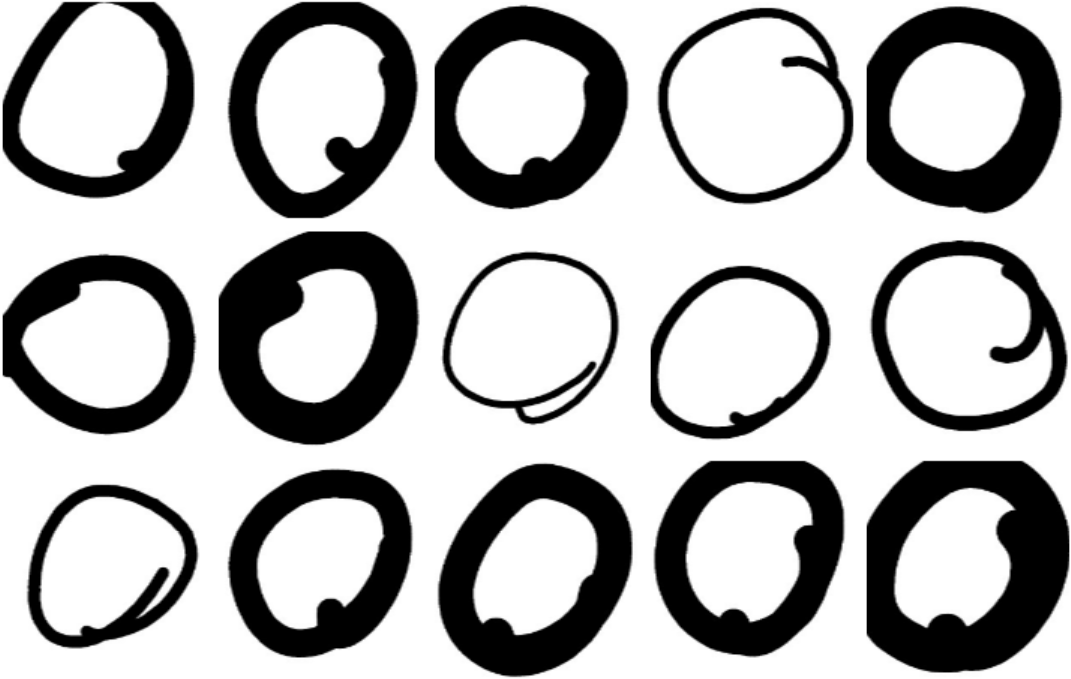
\includegraphics[width=\textwidth]{images/os.png}
        \caption{lose Nodes}
        \label{fig:os}
    \end{subfigure}
    \begin{subfigure}[b]{0.4\textwidth}
        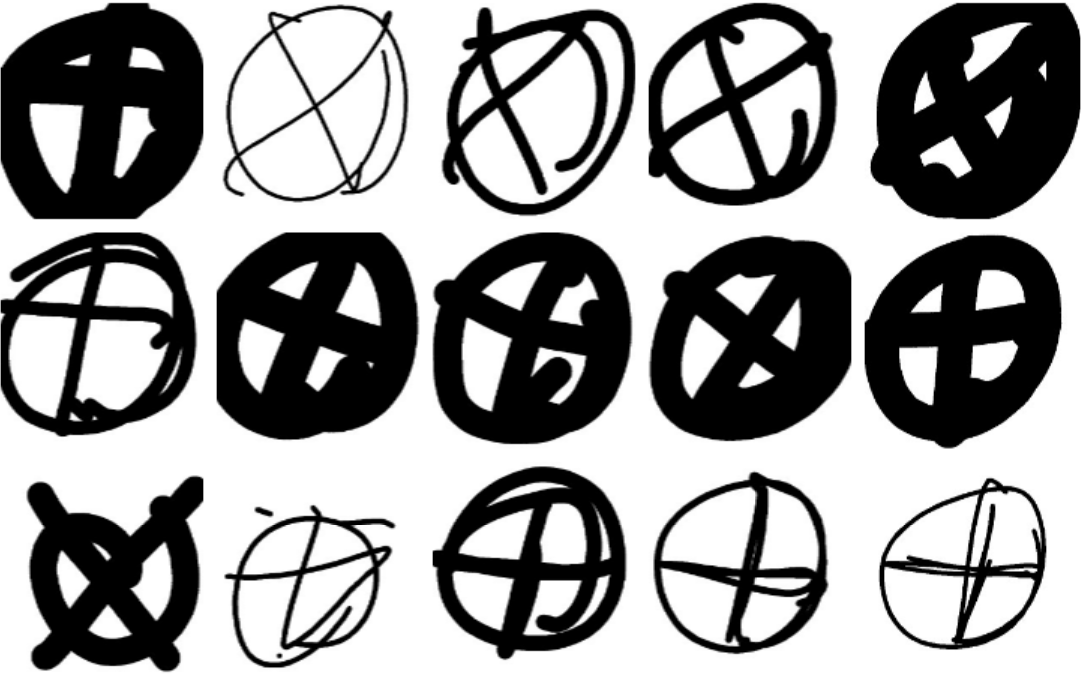
\includegraphics[width=\textwidth]{images/xs.png}
        \caption{Base-Nodes}
        \label{fig:xs}
    \end{subfigure}
    \begin{subfigure}[b]{0.4\textwidth}
      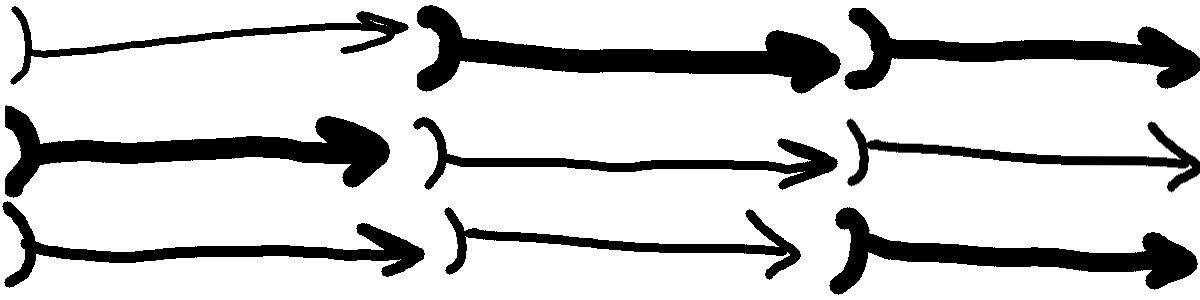
\includegraphics[width=\textwidth]{images/rs.png}
      \caption{rotatorische Constraints}
      \label{fig:rs}
    \end{subfigure}
    \begin{subfigure}[b]{0.4\textwidth}
      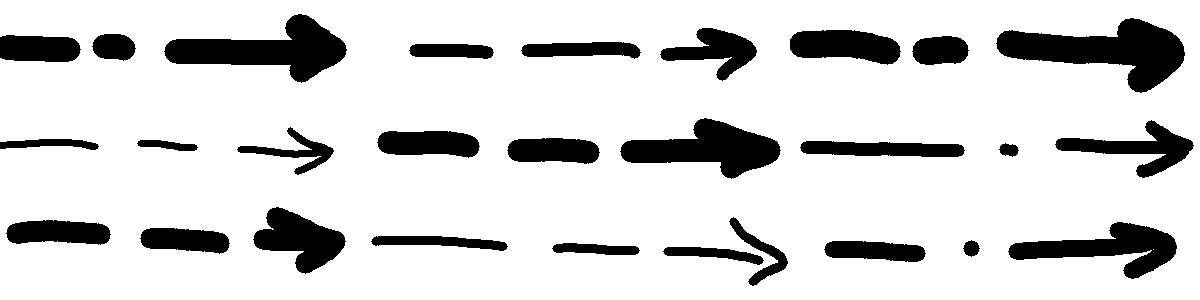
\includegraphics[width=\textwidth]{images/ts.png}
      \caption{translatorische Constraints}
      \label{fig:ts}
    \end{subfigure}
    \caption{Beispiele für handgezeichnete Symbole welche zum Trainieren der Algorithmen genutzt werden.}
    \label{fig:example_symbols}
\end{figure}

Neben den Nodes wurden für die Constraints wieder 1200 rotatorische und 1200 translatorische Verbindungen gezeichnet, welche sich in ihrer Gestaltung an die Darstellung von Constraints an Abbildung \ref{fig:constraints_gtk} orientieren.
Für gebundene und freie Constraints gibt es noch keine Trainingsdaten, da diese für die momentan bestimmte Funktion zunächst irrelevant sind.

\begin{figure}
  \centering
  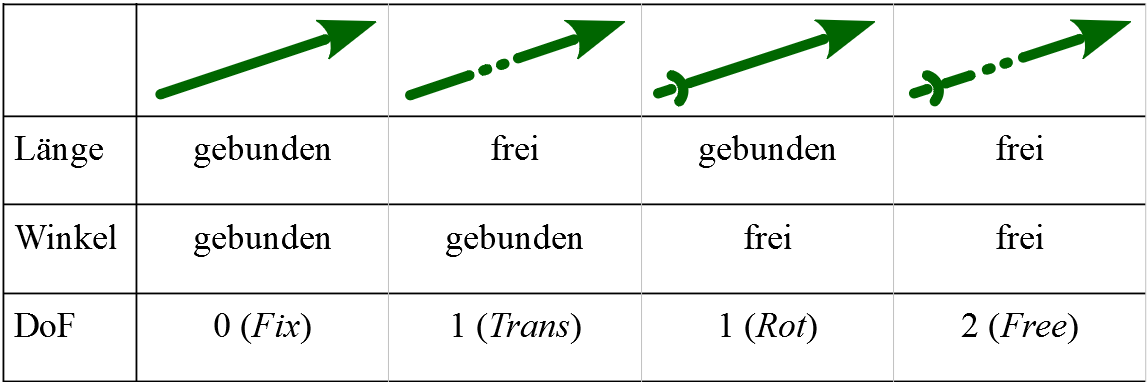
\includegraphics[width=0.8\textwidth]{images/gtk2019_tab1.png}
  \caption{Darstellung der Constraints in ihren unterschiedlichen Auslagemöglichkeiten. Auszug von Tabelle 1 des Beitrags von Prof. Gössner zum Sammelband des Getriebetechnischen Kolloquiums 2019 in Dortmund\cite{Goessner2019a}}.
  \label{fig:constraints_gtk}
\end{figure}


\printbibliography

\end{document} 